\section{EJERCICIO 2.1: Utilizar conversor BCD}
\sangria{} La consigna de este ejercicio es utilizar un conversor BCD a 7 segmentos CD4511 con el minilab. Se hace enfasis en que se debe aprovechar todo el potencial del integrado, especialmente las entradas de control $LE$, $\overline{BI}$ y $\overline{LT}$.

\subsection{El decodificador BCD}

\sangria{} Este decodificador toma como entrada un número en forma binaria  y luego forma en su salida la secuencia exacta para representar ese número binario en el display, transformado a base decimal.

\begin{center}\begin{figure}[h!]
\centering
\begin{subfigure}[b]{0.65\linewidth}
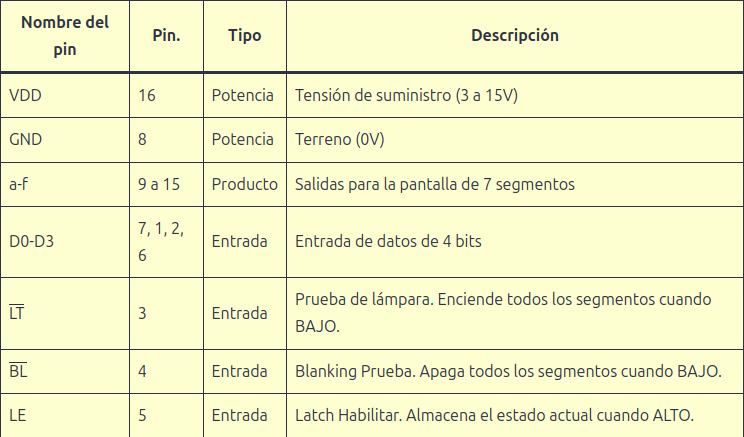
\includegraphics[width=\linewidth]{./fotosAcevedo/pines.png}
% \caption{Identificación de pines}
\label{fig:westminster_lateral}
\end{subfigure}
\begin{subfigure}[b]{0.3\linewidth}
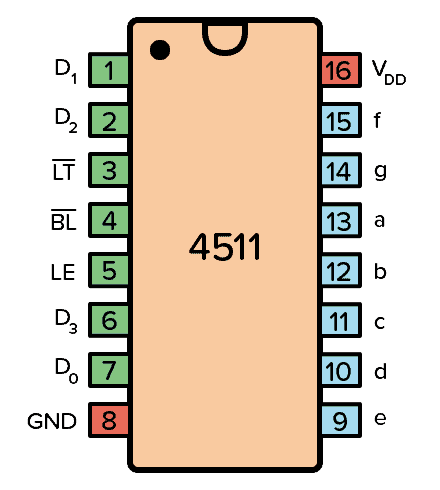
\includegraphics[width=\linewidth]{./fotosAcevedo/PINOUT_4511.png}
% \caption{1 - CPLD}
\label{fig:westminster_aerea}
\end{subfigure}
\caption{Pines del CD4511}
\label{fig:westminster}
\end{figure}\end{center}

\subsection{Materiales usados}

\begin{itemize}[nosep]
    \item Mini laboratorio (minilab) 
    \item Decodificador BCD a 7 segmentos CD4511 
    \item Resistores (para limitar la corriente al display) 
    \item Display de 7 segmentos 
    \item Fuente de alimentación $V_{CC}$ 
    \item Cables Dupont
\end{itemize}

\subsection{Procedimiento}

\begin{enumerate}[nosep]
    \item Se analizó el datasheet del $CD4511$.
    \item Se armó el circuito siguiendo el esquemático. Identificando los pines del decodificador BCD a 7 segmentos y el display según fabricante.
    \item Se colocaron las resistencias limitadoras de corriente al display de 7 segmentos.
    \item Se energizó el circuito con la fuente de alimentación.
    \item Proporcionamos una entrada en formato BCD de 4 bits al decodificador y se observó el resultado en el display.
\end{enumerate}
\newpage
\sangria{} El siguiente esquemático representa la conexión realizada:
\imagen[Esquemático]{15cm}{./fotosAcevedo/ESQUEMATICO_DATASHET.png}
\sangria{} Los interruptores que aparecen pertenecen a las llaves selectoras del minilab empleado.
\imagen[Implementación]{10cm}{./imagenes/causaMinilabBCD.jpg} 

\subsection{Preguntas de análisis}

\begin{enumerate}
    \item \textbf{¿Cuál es la función del decodificador BCD a 7 segmentos?}\\ 
        \sangria{} El decodificador CD4511 es un circuito integrado BCD (decimal codificado a binario) a siete segmentos que permite mostrar valores numéricos en un display usando de entrada un código BCD. Sirve como ''traductor'' de instrucciones (combinaciones binarias de 4 bits 0000-1001) en las señales adecuadas para activar segmentos del display, de modo que se muestre el digito correspondiente del 0 al 9. 
    \item \textbf{¿Cuál es la conexión adecuada entre el decodificador y el display de 7segmentos?}\\ 
        \sangria El integrado CD4511 posee 4 entradas de datos: \textbf{D C B A} para el código en BCD. Posee siete salidas: $a \rightarrow g$ que controlan los segmentos del display. Cuenta con entradas de control (LATCH ENABLE), BLANKING y LAMP TEST que permiten almacenar de forma tempotal un valor, apagar el display sin perder el dato o encender todos los segmentos simultáneamente. 
        % \imagen[Distribución de pines CD4511]{7cm}{./imagenes/pinesCD4511.png}

    \item \textbf{¿Qué sucede si se proporciona una entrada inválida al decodificador?}\\ 
        \sangria{} Dicho escenario se responde mirando la tabla de verdad del decodificador CD4511: 
\begin{center}
\begin{tabular}{|
>{\columncolor[HTML]{FFCCC9}}l |l|l|l|l|l|l|l|l|l|l|l|}
\hline
\cellcolor[HTML]{B0F6F2}\textbf{Decimal} & \cellcolor[HTML]{B0F6F2}\textbf{D3} & \cellcolor[HTML]{B0F6F2}\textbf{D2} & \cellcolor[HTML]{B0F6F2}\textbf{D1} & \cellcolor[HTML]{B0F6F2}\textbf{D0} & \cellcolor[HTML]{B0F6F2}\textbf{a} & \cellcolor[HTML]{B0F6F2}\textbf{b} & \cellcolor[HTML]{B0F6F2}\textbf{c} & \cellcolor[HTML]{B0F6F2}\textbf{d} & \cellcolor[HTML]{B0F6F2}\textbf{e} & \cellcolor[HTML]{B0F6F2}\textbf{f} & \cellcolor[HTML]{B0F6F2}\textbf{g} \\ \hline
\rowcolor[HTML]{EFEFEF}\cellcolor[HTML]{FFFFC7}0 & 0 & 0 & 0 & 0 & 1 & 1 & 1 & 1 & 1 & 1 & 0 \\ \hline
\rowcolor[HTML]{EFEFEF}\cellcolor[HTML]{FFFFC7}1 & 0 & 0 & 0 & 1 & 0 & 1 & 1 & 0 & 0 & 0 & 0 \\ \hline
\rowcolor[HTML]{EFEFEF}\cellcolor[HTML]{FFFFC7}2 & 0 & 0 & 1 & 0 & 1 & 1 & 0 & 1 & 1 & 0 & 1 \\ \hline
\rowcolor[HTML]{EFEFEF}\cellcolor[HTML]{FFFFC7}3 & 0 & 0 & 1 & 1 & 1 & 1 & 1 & 1 & 0 & 0 & 1 \\ \hline
\rowcolor[HTML]{EFEFEF}\cellcolor[HTML]{FFFFC7}4 & 0 & 1 & 0 & 0 & 0 & 1 & 1 & 0 & 0 & 1 & 1 \\ \hline
\rowcolor[HTML]{EFEFEF}\cellcolor[HTML]{FFFFC7}5 & 0 & 1 & 0 & 1 & 1 & 0 & 1 & 1 & 0 & 1 & 1 \\ \hline
\rowcolor[HTML]{EFEFEF}\cellcolor[HTML]{FFFFC7}6 & 0 & 1 & 1 & 0 & 1 & 0 & 1 & 1 & 1 & 1 & 1 \\ \hline
\rowcolor[HTML]{EFEFEF}\cellcolor[HTML]{FFFFC7}7 & 0 & 1 & 1 & 1 & 1 & 1 & 1 & 0 & 0 & 0 & 0 \\ \hline
\rowcolor[HTML]{EFEFEF}\cellcolor[HTML]{FFFFC7}8 & 1 & 0 & 0 & 0 & 1 & 1 & 1 & 1 & 1 & 1 & 1 \\ \hline
\rowcolor[HTML]{EFEFEF}\cellcolor[HTML]{FFFFC7}9 & 1 & 0 & 0 & 1 & 1 & 1 & 1 & 0 & 1 & 1 & 1 \\ \hline
\end{tabular}
\end{center}
        \sangria{} Cuando se ingresa un valor binario existente en la tabla, se activan las salidas correspondientes para formar el digito en el display, para cualquier otro valor incorrecto (ej: mayor que 1001), el decodificador apaga el display poniendo sus salidas a 0 (los ''Blank''). 
    \item \textbf{¿Cuál es la relación entre los bits de entrada y los segmentos del display?}\\ 
        \sangria{}Es lógica y combinacional: cada segmento de salida ($a,b,c,d,e,f,g$) responde a una función booleana individual determinada por 4 bits de código de BCD. El decodificador traduce cada valor binario en el patrón específico para encender los segmentos del display. Para los minitérminos $m_{10}$ al $m_{15}$ el decodificador pone a $0$ todas las salidas.
    \item \textbf{¿Cuál es la utilidad de los resistores del circuito?}\\
        \sangria{} Los resistores permiten limitar la corriente directa que llega a los leds que conforman el display de 7 segmentos. Dado que un led tiene una curva tensión-corriente exponencial una vez superada la tensión umbral $V_F \approx 2V$, lo que provocaría que le demande más corriente a la fuente y termine quemando el display. Se dispone un resistor por cada segmento.
\end{enumerate}

\subsection{Conclusiones}
\sangria{} Se comprobó la tabla de verdad de los pines de entrada del decodificador para visualizar las combinaciones del display de 7 segmentos sin inconvenientes complejos. Se ha tomado un tiempo extenso en instalar las conexiones.
